% Document type and paper size
\documentclass[12pt,a4paper]{report}

% Fonts and Typography
\usepackage{newtxtext}
\usepackage[none]{hyphenat}
\usepackage{ragged2e}
\justifying

% Formatting and Layout 
\usepackage{geometry}
\geometry{margin=1in}
\usepackage{setspace}
\setstretch{1.5}
\setlength{\parindent}{1.5em} 
\setlength{\parskip}{0em} 
\setcounter{secnumdepth}{3} 

% Encoding and Hyperlinks
\usepackage[utf8]{inputenc}
\usepackage{hyperref}

% Headers and Footers
\usepackage{fancyhdr}
\pagestyle{fancy}
\fancyhf{} 
\fancyhead[L]{\leftmark} 
\fancyhead[R]{\thepage}            
\fancyfoot{}
\renewcommand{\chaptermark}[1]{\markboth{Chapter \thechapter\ - #1}{}}

% Table of Contents, Bibliography, and Lists
\usepackage{tocbibind}
\usepackage{tocloft} 

% Formatting and Layout 
\usepackage{geometry}
\geometry{margin=1in}
\usepackage{setspace}
\setstretch{1.5}
\setlength{\parindent}{1.5em} 
\setlength{\parskip}{0em} 
\setcounter{secnumdepth}{3}
\setlength{\parskip}{1em} 
\setlength{\textfloatsep}{0.5em}

% Titles Formatting
\usepackage{titlesec}  
\titleformat{\chapter}[block]
  {\normalfont\huge\bfseries\centering}
  {Chapter \thechapter}
  {0pt}
  {\vspace{1em} \\}
\titlespacing*{\chapter}{0pt}{-30pt}{20pt}
% Add a 1-line space before and after the section title
\titlespacing*{\section}{0pt}{\baselineskip}{\baselineskip}

% Figures and Graphics
\usepackage{graphicx}
\usepackage{subfig} 
\usepackage{caption}
\usepackage{float}

% Lists and Enumerations
\usepackage{enumerate}
\usepackage{enumitem}
\setlist[enumerate,1]{label=\alph*., leftmargin=2em} 

% Mathematical Tools, algorithms
\usepackage{algorithm}
\usepackage{algpseudocode}
\usepackage{amsmath}

% Tables
\usepackage{xcolor}
\usepackage{colortbl}
\usepackage{booktabs} 
\usepackage{multirow} 
\usepackage{array}    
\usepackage{siunitx}  
\usepackage{makecell}
\usepackage{tabularx} 


% Glossaries and Acronyms
\usepackage{acronym}
\usepackage[acronym]{glossaries}

%%%%%%%%%%%%%%%%%%%%%%%%%%%%%%%%%%%%%%%%%%%%%%%%

\begin{document}
% Title Page
\begin{titlepage}
    \begin{center}
        \vspace*{-0.05cm} % Lift the content up
        
\includegraphics[width=0.2\textwidth]{Figures/Fig:logo.jpg}\\[1cm]  % Adjusted spacing
        {\Large\textbf{This is the Thesis Title}}\\[0.5cm]
        {\large \textit{A thesis submitted in partial fulfillment of the requirements of the B.Sc. degree in Electrical and Electronic Engineering}}\\[1.5cm]
        \begin{spacing}{1.5}  % Set line spacing to 1.5
        \textbf{Submitted by:}\\[0.5cm]
        {\textbf{Student Name (Index)}}\\
        {\textbf{Student Name (Index)}}\\[1cm]
        \textbf{Supervised by:}\\[0.5cm]
        {\textbf{Supervisor name}}\\[1cm]
        \textbf{To}\\[0.5cm]
        {\textbf{Department of Electrical and Electronic Engineering}}\\
        {\textbf{Faculty of Engineering}}\\
        {\textbf{University of Khartoum}}\\[1.5cm]
        \textbf{September 2024}
        \end{spacing}
    \end{center}
\end{titlepage}

% Start of the Content
\pagenumbering{roman}
\chapter*{Declaration of Authorship}


You can check the official EEE department thesis guidelines from the main menu \textbf{"thesis Guidelines .pdf "}

\section*{Note}
This templete doesn't support Arabic language yet, so you can't write your arabic version of abstract. 

I'll update it as soon as possible!
\chapter*{Dedication}
\vspace{2em}
\chapter*{Acknowledgments}
\vspace{2em}
\chapter*{Abstract}
\vspace{2em}
\chapter*{\centering\textarabic{الملخص}}
\vspace{2em}
\begin{Arabic}
هذا نص بالعربي
\end{Arabic}

\listoftables
\newpage
\listoffigures
\newpage
\tableofcontents
\chapter*{List of Abbreviations}
\addcontentsline{toc}{chapter}{List of Abbreviations}
\begin{acronym}[LONGEST]

\acro{TE}{\textbf{T}est \textbf{E}xample} 

\acro{AE}{\textbf{A}nother \textbf{E}xample} 

% Give this fromat and all of your acronyms to any AI tool with  :)

\end{acronym}

\pagenumbering{arabic}
\chapter{Introduction}
\vspace{2em}

\paragraph{General guidelines page :) }

% To add a new Title, use the 'hash section' as shown below: 

\section{Overview}
Write your paragraph here.

To start another paragraph, keep an empty line.
If you don't, it will continue in the same line.

\section{Problem Statement}
\section{Literature Review}
\section{Objectives}

%to add a numbered list, use the following code:
This is a numbered list:
\begin{enumerate}
    \item the first item
    \item the second item
\end{enumerate}

\section{Methodology}
This is a bullet list: 
\begin{itemize}
    \item the first item
    \item the second item
\end{itemize}

\section{Thesis Layout}

This is another bullet list: 
\begin{itemize}[label=-]
    \item the first item
    \item the second item
\end{itemize}
\chapter{Theoretical Background and Literature Review}
\section{This is the First Title in Chapter 2}

To add a citation, use the "hash cite" and add your reference from 'References.bib' as shown below:
This is The first reference \cite{yao2024survey}

For adding a subtitle and sub-subtitle, use "hash subsection" and "hash subsubsection" as shown below: 

\subsection{This is the First Subtitle}

The term \ac{TE} is used in this document.
The term \ac{AE} is used in this document.

\subsubsection{This is the First sub-subtitle}

The  main aim of this chapter:
\begin{enumerate}
    \item Group research studies according to common Denominators. Point out overall trends in what has been published
    \item Summarize individual studies or articles with as much or as little detail as each merits. Build research citations on each other.
    \item  Summarize major contributions of significant studies and articles to the body of knowledge under review.
    \item Evaluate the current "state of the art" for the body of knowledge reviewed,
\end{enumerate}
\chapter{Methodology}
\vspace{2em}
\section{Adding a Figure}

%To add a figure, upload your png and use the following code: 

%%%%%%%%%%%%%%%%%%%%%%%%%%%%%%%%%%%%%%%%%%%
\begin{figure}[H]
    \centering
    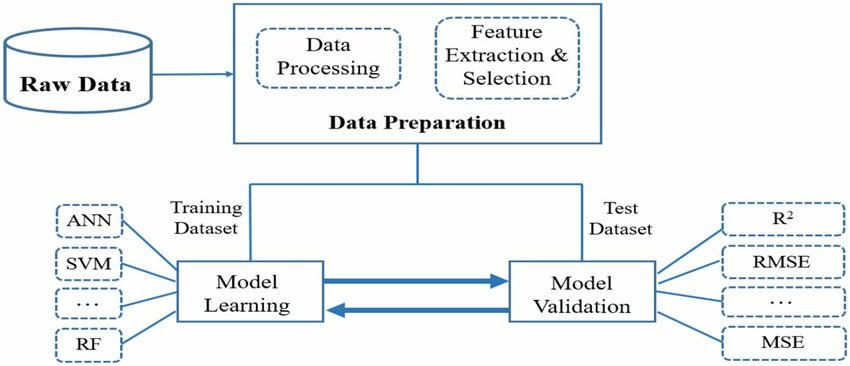
\includegraphics[width=0.8\textwidth]{Figures/Fig:ML-workflow.png}
    \caption{Machine Learning Model Development Workflow}
    \label{fig:ml-workflow}
\end{figure}
%%%%%%%%%%%%%%%%%%%%%%%%%%%%%%%%%%%%%%%%%%%

% Add your figure in "include graphic {} brackets", and you can modify the size from "width"

% Add your figure title in "caption {} brackets" 

% Add your figure label in the "label {} brackets"

% You can mention your figure in any paragraph through the label using the "hash ref" as shown below:

ML model development requires several key steps, as illustrated in Figure~\ref{fig:ml-workflow}.
\chapter{Results and Discussion}
\vspace{2em}

\section{Adding a teble}

In the same way as in figures, you can mention any table through it's label using the "hash ref" as showing below:

The results are summarized in Table~\ref{tab:comparison}. Each method has its strengths and weaknesses, which are analyzed below.

% For adding a table, use the following code: 

\begin{table}[htbp] 
    \centering
    \caption{Comparison of Different Methods} %This is the title of the table
    \label{tab:comparison}
    \begin{tabular}{@{}lccc@{}}
        \toprule
        \textbf{Method} & \textbf{Accuracy (\%)} & \textbf{Processing Time (ms)} & \textbf{Memory Usage (MB)} \\
        \midrule
        Method A & 95.2 & 120 & 256 \\
        Method B & 93.8 & 85 & 312 \\
        Method C & 97.1 & 150 & 428 \\
        \bottomrule
    \end{tabular}
\end{table}

l\chapter{Conclusion}
\section{Adding an algorithm}

 USE ANY AI TOOL TO GENERATE LATEX CODE OF ALGORITHMS AND EQUATIONS SO YOU CAN GAIN TIME 

\subsection{Adding an algorithm}

\begin{algorithm}
\caption{Example Algorithm}
\begin{algorithmic}[1]  % The number 1 here means that the lines will be numbered
\State Initialize $x \gets 0$
\For{$i = 1$ to $n$}
    \State $x \gets x + i$
\EndFor
\State \textbf{Return} $x$
\end{algorithmic}
\end{algorithm}

\subsection{Adding an equation}
%You can use ChatGPT to generate each eqatiuon code :)
        \begin{equation}
        \text{A} = \frac{B}{C + D} 
        \label{first_eq}
        \end{equation}
        
You can mention it in any part of the text through it's label using the "hash ref" as shown below 

As shown in equation ~\ref{first_eq} %ADD THE LABEL HERE
\bibliographystyle{IEEEtran} 
% Choose a citation style (e.g., IEEE, APA, plain, etc.)
\bibliography{References}
% This should match your .bib file name

\end{document}




